
We have to convert the pose that we managed to estimate, into a file that animator software can read. We choose to convert it into a BVH file, as it is the most common file for computerized mocap clips. \\

Firstly, we have to create a skeleton in BVH form. This skeleton must be identical to the skeleton of the datasets that our model used. Therefore we created in python a skeleton with 17 main bones and 4 limb bones that follow the movement of their parent bone. We also initialized the first frame of the movement as a T-Pose, to make the motion retarget easier for the animators.\\

In the BVH format, the following relationship holds between the joints:
$$orientation_j=R_{P(j)}offset_j + orientation_{P(j)}$$

where $orientation_j$ indicates the 3D orientation of joint j, P(j) returns the parent of joint j in whatever DAG (directed acyclic graph) the orientations are modeled in (generally the DAG starts at the root and points towards the end-effectors) $offset_j$ indicates the offset of joint j relative to its parent P(j) (aka the connecting limb), and $R_{P(j)}$ is the 3D rotation that determines how much should $offset_j$ be rotated from an initial pose (generally a T-pose). In the BVH format, for each parent P(j), we need to store $R^{-1}_{P(j)}R_j$. The main problem was working with joints that had multiple children, for example, the root joint, which has connections to both legs as well as the spine. Therefore, we came up with a solution for joints with multiple children, I had to make copies with offset=0, and assign those as parents of the corresponding chains. \\

Regarding the position of the humanoid, which in our case only only the hip has, we can easily convert it. We assume that the hip starts in the frame 0 in the location (0, hipSkeletonHeight, 0) , so with this point as a reference, we can perfectly convert the position into an computerized space that the animators will use.\\

\begin{figure}[htp]
    \centering
    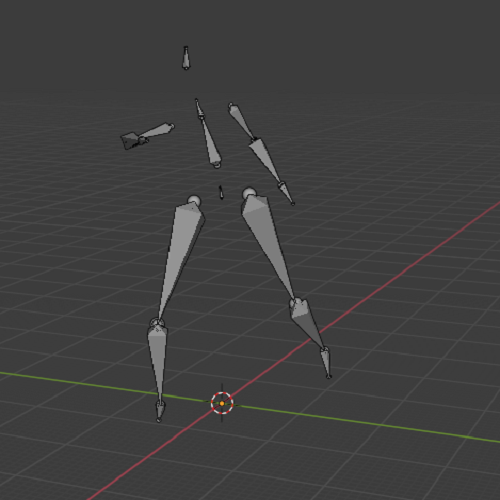
\includegraphics[width=5cm]{figures/Implementation/skeleton1.png}%
    \qquad
    \includegraphics[width=5cm]{figures/Implementation/skeleton2.png}%
    \qquad
    \includegraphics[width=5cm]{figures/Implementation/skeleton3.png}%
    \qquad
    \includegraphics[width=5cm]{figures/Implementation/skeleton4.png}%
    \captionsetup{labelformat=empty}
    \caption{The results of the BVH File from a video when we import it into Blender. The same frame from different camera positions.}%
    \label{fig:example}%
\end{figure}

Finally, we completed the first phase of our goal, we estimated the 6D human pose, or we estimated the orientation and the location of the human in the video for each frame and we convert it into a BVH file. Subsequently, we will discuss about some ways that will improve these results 


